% NOX-008 — Spatial-scale & autocorrelation-robust sensitivity of the NO2<->steel signal.
% Self-contained working paper for the NOXUS project. Compile with:
%     pdflatex nox008_spatial_scale.tex   (run twice for references/labels)
% Figures are produced by analysis/nox008_spatial_scale.py and read from
% ../docs/figures/nox008/.
\documentclass[11pt,a4paper]{article}

\usepackage[utf8]{inputenc}
\usepackage[T1]{fontenc}
\usepackage{lmodern}
\usepackage[margin=2.4cm]{geometry}
\usepackage{graphicx}
\usepackage{booktabs}
\usepackage{amsmath}
\usepackage{caption}
\usepackage{subcaption}
\usepackage{xcolor}
\usepackage[round,authoryear]{natbib}
\usepackage[hidelinks]{hyperref}
\usepackage{authblk}
\usepackage{enumitem}

\graphicspath{{../docs/figures/nox008/}{../docs/figures/preliminary/}{../docs/figures/exploration/}}
\captionsetup{font=small,labelfont=bf}
\setlength{\parskip}{0.35em}

% Lightweight replacements for siunitx (this MiKTeX kernel is too old for it).
\providecommand{\degree}{\ensuremath{^{\circ}}}
\newcommand{\SI}[2]{#1\,#2}
\newcommand{\rval}[1]{\mbox{$r=#1$}}

\title{\bfseries A designed null at every scale: spatial-scale and
autocorrelation-robust sensitivity of a satellite-\ce{NO_2} steel-activity signal
for the Tangshan cluster}

\author[1]{A.~Betato}
\affil[1]{NOXUS project --- \texttt{abetatos@gmail.com}}
\date{NOX-008 working paper \quad\textbullet\quad 14 June 2026}

% A tiny bit of chemistry notation without mhchem (works in text and math).
\providecommand{\ce}[1]{\ensuremath{\mathrm{#1}}}

\begin{document}
\maketitle

\begin{abstract}
\noindent
The NOXUS pipeline turns Sentinel-5P/TROPOMI tropospheric \ce{NO_2} over the Tangshan
(Hebei) steel cluster into a relative steel-activity signal and tests it against the
CREA blast-furnace (BF) operating-rate benchmark. Earlier phases reported an apparent
\emph{decoupling}: on a partial \ce{NO_2} cube the meteorology-normalised cluster signal
correlated negatively with the BF rate in levels (monthly \rval{-0.35}) and only weakly
after detrending. Two suspicions remained: that the result was an artefact of a single
fixed \emph{spatial scale}, and that the significance was inflated by treating strongly
\emph{autocorrelated} monthly series as i.i.d. This paper (NOX-008) resolves both on the
complete, rebuilt 389-week cube (2019--2026). We sweep two scale axes by aggregation
only --- area-of-interest (AOI) extent (\SI{0.25}{\degree} vs \SI{0.10}{\degree} buffer)
and grid resolution (native \,$\sim$\SI{0.04}{\degree}, block-averaged $\sim$\SI{0.1}{\degree}
and $\sim$\SI{0.25}{\degree}) --- and re-judge every correlation with an
autocorrelation-aware test: first-order effective sample size, a moving-block bootstrap
confidence interval, a block-permutation null, and a Benjamini--Hochberg
multiple-testing correction across the whole grid. The result is an emphatic, designed-for
null: across $16$ scale\,$\times$\,variant cells, \textbf{zero} are significant even at the
naive $p<0.05$ threshold and \textbf{zero} survive the autocorrelation-robust test; the
sign of the levels relationship is itself unstable across scale ($-,+,-,-$); and the
coarsest grid cannot resolve a source/background contrast at all. The full series collapses
the partial-cube $-0.35$ to $-0.05$. We conclude that the weak/null \ce{NO_2}$\leftrightarrow$BF
coupling is not an artefact of one scale or of an over-optimistic significance test: it is
robust to both. This hardens the project conclusion from ``no signal at one scale'' to
``no robust signal at any reasonable scale,'' and motivates the two remaining levers ---
a diurnal geostationary sensor (GEMS) and flux-divergence point-source attribution.
\end{abstract}

\section{Background and antecedents}
\label{sec:background}

\paragraph{The premise.} Satellite \ce{NO_2} is an established proxy for combustion activity,
and a small literature uses it as an economic nowcast: at national scale for China
\citep{morris_zhang_2019,li_zheng_2023,li_2024_nox_trends}, across global cities
\citep{montgomery_holloway_2018}, and as a war/industrial-shock read for Ukraine
\citep{mao_2025_ukraine}; the broad case for satellite data in economics is made by
\citet{donaldson_storeygard_2016} and \citet{ezran_2023}. NOXUS asks a deliberately harder,
single-cluster question: can the \ce{NO_2} column over one industrial cluster --- the
Tangshan blast-furnace complex, the largest steel agglomeration in China --- track that
cluster's physical output at a useful frequency, using only public, free data?

\paragraph{The NOXUS arc.} Prior phases built the machinery and tested it honestly:
NOX-001 ingested the CREA Tangshan BF operating-rate benchmark \citep{crea_steel_benchmark};
NOX-002 acquired TROPOMI \ce{NO_2} over the AOI via openEO and composited it into an
analysis-ready weekly cube; NOX-003 derived a relative steel-activity signal using the
cluster/relative-index paradigm \citep{kim_2023}, with the dominant ventilation confounder
regressed out via ERA5 winds and boundary-layer height
\citep{hersbach_2020_era5,cds_era5,li_2024_nox_trends}. NOX-003 returned an
\emph{honest near-null}: in levels the cluster signal correlated \emph{negatively} with the
BF rate (monthly $\sim-0.35$), the fingerprint of \emph{decoupling} --- emission intensity
(\ce{NO_x} per tonne) falling secularly faster than activity rises, driven by
ultra-low-emission retrofits and policy \citep{li_2024_nox_trends}. NOX-003.1 modelled that
intensity trend explicitly and confirmed only a weak positive residual relationship
($r\!\sim\!0.14$, below the pre-registered $0.5$--$0.75$ bar). NOX-004 reframed the signal as
a discrete \emph{event} marker rather than a continuous tracker, and NOX-006 added a daily
Prophet decomposition to exploit the weekly cycle for source separation --- which TROPOMI's
single $\sim$13:30 overpass renders invisible (weekly term flat, $0.5\%$ of variance).
A decisive full-series \emph{arbiter} re-ran the chain on the complete, rebuilt 389-week cube
and found the average coupling collapses (weekly \rval{0.07}, monthly \rval{0.13}), with a
regime-dependent rolling peak. The full series does not rescue the signal.

\paragraph{Two unresolved suspicions.} Every prior number was computed at a \emph{single}
spatial scale --- one AOI buffer, one native grid --- and judged with the \texttt{scipy}
Pearson $p$-value, which assumes independent observations. Both choices can manufacture or
destroy a correlation:
\begin{enumerate}[leftmargin=1.4em,itemsep=0.2em]
  \item \textbf{Scale.} \citet{parubets_naito_2025} show, for Japanese local economic
  indicators, that an \ce{NO_2}$\leftrightarrow$activity correlation that is significant at a
  coarse spatial scale can weaken, vanish, or flip sign at a finer one. Steel is only
  $\sim$30--43\% of Tangshan's \ce{NO_2} column \citep{scirep_2024}; a tighter AOI might
  isolate the source from the Beijing--Tianjin--Hebei background, or a coarser grid might
  average the cluster into that background.
  \item \textbf{Serial dependence.} \ce{NO_2} and the BF rate are smooth, strongly
  autocorrelated series. The effective number of independent observations is far below the
  nominal $n$, so a naive $p$-value and the $\pm1.96/\sqrt{n}$ lead-lag band overstate
  significance \citep{morris_zhang_2019}.
\end{enumerate}

\paragraph{This paper.} NOX-008 confronts both suspicions on the complete cube. We sweep
extent and resolution by \emph{aggregation only} (never interpolation to a finer grid) and
re-judge every correlation with an autocorrelation-robust test and a multiple-testing
correction across the whole scale grid. An honest null is an acceptable, designed-for outcome
\citep{morris_zhang_2019}; the contribution is to show \emph{how robust} that null is.

\section{Data}
\label{sec:data}

\paragraph{Tropospheric \ce{NO_2} cube.} The analysis-ready product is the NOX-002b weekly
composite cube (\texttt{no2\_cube\_w.nc}): $30\times51$ cells at native
$\sim$\SI{0.035}{\degree}\,$\times$\,\SI{0.055}{\degree} ($\sim$\SI{4}{}--\SI{6}{km}),
$389$ weekly slots spanning 2019-01-06 to 2026-06-14, with per-cell valid-coverage tracked
and cloud-gapped cells left as \texttt{NaN} (never interpolated). The AOI is \emph{derived}
from the located steel facilities (GEM Global Iron \& Steel Tracker): the bounding envelope
of all TROPOMI-era integrated BF/BOF plants in Tangshan prefecture
(\SI{117.964}{}--\SI{119.047}{\degree}E, \SI{38.954}{}--\SI{40.210}{\degree}N), expanded by a
configurable buffer.

\paragraph{Physical-output benchmark.} The CREA Tangshan blast-furnace operating-rate series
\citep{crea_steel_benchmark} --- weekly, WIND-sourced, republished freely by CREA --- is the
ground truth. It rises secularly across the window (Fig.~\ref{fig:decoupling}, blue), the
hallmark of recovering and consolidating output.

\paragraph{Meteorology.} ERA5 single-levels 10\,m wind ($u_{10},v_{10}$) and boundary-layer
height (\texttt{blh}) at the overpass window \citep{hersbach_2020_era5,cds_era5}, aggregated
over the footprint and regressed out of the cluster signal as the dominant ventilation
confounder \citep{li_2024_nox_trends}. The meteorological covariate is regional and
\emph{scale-independent}, so the identical covariate set is applied at every spatial scale.

\section{Methods}
\label{sec:methods}

\subsection{Signal chain (canonical, per scale)}
For each spatial scale we reproduce the NOX-003 chain exactly. (i) \textbf{Footprint--background
contrast}: select cube cells within a haversine radius of any operating facility (the
footprint), and an annular background ring around the cluster centroid clipped to the AOI;
the signal is the per-week footprint mean minus the background mean. (ii) \textbf{Meteo
regress-out}: OLS-residualise the footprint signal on the ERA5 covariates
$\{u_{10},v_{10},\texttt{blh},\text{wind speed}\}$. (iii) \textbf{Deseason variants}: from the
meteo-free monthly series we build four representations --- \textsf{level} (no detrending),
\textsf{intensity} (explicit smoothness-controlled secular-trend residual, the NOX-003.1
decoupling model), \textsf{yoy} (year-over-year difference), and \textsf{stl} (STL residual).
Each is aligned to the monthly BF rate and correlated at lag $0$ and at its peak-$|r|$ lead-lag
($\pm8$ months).

\subsection{Two scale axes (aggregation only)}
\label{sec:axes}
\textbf{Axis 1 --- AOI extent.} A strict spatial clip of the cube to the facility envelope plus
a buffer: \textsf{wide} \SI{0.25}{\degree} ($\sim$\SI{28}{km}, the default) vs \textsf{tight}
\SI{0.10}{\degree} ($\sim$\SI{11}{km}). The tight clip tests the source-isolation intuition:
less external background, but also fewer cells.
\textbf{Axis 2 --- grid resolution.} Block-averaging the cube by integer factors over $(y,x)$
via \texttt{xarray.coarsen} (mean over cell blocks): \textsf{native} $(1,1)$,
\textsf{coarse010} $(3,2)\!\approx\!$\SI{0.1}{\degree}, and \textsf{coarse025}
$(7,5)\!\approx\!$\SI{0.25}{\degree}. Coarsening by averaging is the permitted,
information-preserving direction (consistent with the project's native-resolution decision,
which rejected interpolating to a \emph{finer} grid); it is exactly the
\citet{parubets_naito_2025} resolution experiment. The footprint radius and ring floor at the
native config (\SI{15}{km}; \SI{25}{}--\SI{60}{km}) and scale with the cell size so coarse
grids still resolve a non-empty, disjoint geometry where possible.

\subsection{Autocorrelation-robust significance}
\label{sec:significance}
For every cell we report, alongside the naive Pearson $r$ and $p$:
\begin{itemize}[leftmargin=1.4em,itemsep=0.15em]
  \item \textbf{Effective sample size} $n_{\text{eff}}=n\,(1-ab)/(1+ab)$, with $a,b$ the lag-1
  autocorrelations of the two series (Bayley--Hammersley first order), and the $p$-value
  recomputed on $n_{\text{eff}}-2$ degrees of freedom.
  \item \textbf{Moving-block bootstrap} 95\% CI for $r$ (block length $\lceil n^{1/3}\rceil$,
  $5000$ resamples of the \emph{paired} series, preserving within-block memory).
  \item \textbf{Block-permutation} null $p$: reorder contiguous blocks of $x$ against a fixed
  $y$, destroying the cross-correlation while approximately preserving each series'
  autocorrelation ($5000$ draws).
  \item \textbf{Multiple testing}: a Benjamini--Hochberg false-discovery-rate (FDR) correction
  ($q$-values) across the entire scale\,$\times$\,variant grid. A cell is \emph{robust} only if
  $q_{\text{block}}<0.05$ \emph{and} the bootstrap CI excludes zero.
\end{itemize}
The pipeline is reproducible (\texttt{analysis/nox008\_spatial\_scale.py}, seed $20260614$); it
reads only the committed benchmark and the gitignored \ce{NO_2} cube.

\section{Results}
\label{sec:results}

\subsection{No cell is significant at any scale}
Table~\ref{tab:grid} is the full grid. Of the $16$ scale\,$\times$\,variant cells, the largest
lag-0 $|r|$ is $0.19$ (\textsf{wide-coarse010, level}); \textbf{none} reaches even the naive
$p<0.05$ threshold, and after the FDR correction every $q\approx0.99$. The bootstrap CIs all
straddle zero. The peak-$|r|$ lead-lag columns reach $|r|\!\approx\!0.30$--$0.34$, but those are
selected over $17$ candidate lags and are exactly what the block-permutation null is built to
deflate: not one survives. Figure~\ref{fig:heatmap} renders the lag-0 grid; the palette barely
departs from white.

\begin{table}[t]
\centering
\caption{Full scale\,$\times$\,variant grid (monthly; footprint$-$background \ce{NO_2},
meteo-normalised, vs the CREA BF operating rate). $r$, $p$, $n_{\text{eff}}$ and the
moving-block bootstrap 95\% CI are at lag $0$; $q$ is the Benjamini--Hochberg FDR-adjusted
block-permutation $p$ across all $16$ cells; the last column is the peak-$|r|$ lead-lag $r$
(months). \emph{No cell is naive-significant; none is robust.}}
\label{tab:grid}
\small
\begin{tabular}{llrrrrcrl}
\toprule
Scale & Variant & {$n$} & {$r_{0}$} & {$p$} & {$n_{\text{eff}}$} & {boot 95\% CI} & {$q$} & {best lag $r$} \\
\midrule
wide-native     & level     & 90 & -0.049 & 0.648 & 66.7 & $[-0.31,+0.16]$ & 0.99 & $-0.31$ ($-5$) \\
wide-native     & intensity & 90 & +0.126 & 0.236 & 71.9 & $[-0.12,+0.30]$ & 0.99 & $+0.26$ ($+6$) \\
wide-native     & yoy       & 78 & -0.003 & 0.976 & 55.8 & $[-0.40,+0.29]$ & 0.99 & $-0.26$ ($-6$) \\
wide-native     & stl       & 90 & -0.002 & 0.984 & 84.0 & $[-0.22,+0.17]$ & 0.99 & $-0.23$ ($-5$) \\
\addlinespace
wide-coarse010  & level     & 90 & +0.186 & 0.079 & 62.4 & $[-0.07,+0.36]$ & 0.99 & $+0.28$ ($+4$) \\
wide-coarse010  & intensity & 90 & +0.131 & 0.217 & 62.9 & $[-0.13,+0.31]$ & 0.99 & $+0.23$ ($+4$) \\
wide-coarse010  & yoy       & 78 & -0.065 & 0.572 & 54.3 & $[-0.52,+0.24]$ & 0.99 & $-0.30$ ($-6$) \\
wide-coarse010  & stl       & 90 & +0.108 & 0.312 & 77.0 & $[-0.11,+0.27]$ & 0.99 & $+0.24$ ($+6$) \\
\addlinespace
tight-native    & level     & 90 & -0.081 & 0.447 & 66.2 & $[-0.34,+0.13]$ & 0.99 & $-0.34$ ($-5$) \\
tight-native    & intensity & 90 & +0.093 & 0.383 & 71.4 & $[-0.14,+0.26]$ & 0.99 & $+0.27$ ($+6$) \\
tight-native    & yoy       & 78 & -0.031 & 0.790 & 55.3 & $[-0.41,+0.25]$ & 0.99 & $-0.28$ ($-6$) \\
tight-native    & stl       & 90 & +0.019 & 0.859 & 85.6 & $[-0.21,+0.20]$ & 0.99 & $+0.22$ ($+6$) \\
\addlinespace
tight-coarse010 & level     & 90 & -0.007 & 0.948 & 69.1 & $[-0.27,+0.19]$ & 0.99 & $-0.25$ ($-5$) \\
tight-coarse010 & intensity & 90 & +0.048 & 0.653 & 69.6 & $[-0.21,+0.24]$ & 0.99 & $+0.26$ ($+6$) \\
tight-coarse010 & yoy       & 78 & -0.119 & 0.300 & 56.0 & $[-0.49,+0.19]$ & 0.99 & $-0.31$ ($-7$) \\
tight-coarse010 & stl       & 90 & -0.044 & 0.682 & 77.6 & $[-0.31,+0.15]$ & 0.99 & $-0.21$ ($-5$) \\
\bottomrule
\end{tabular}
\end{table}

\begin{figure}[t]
\centering
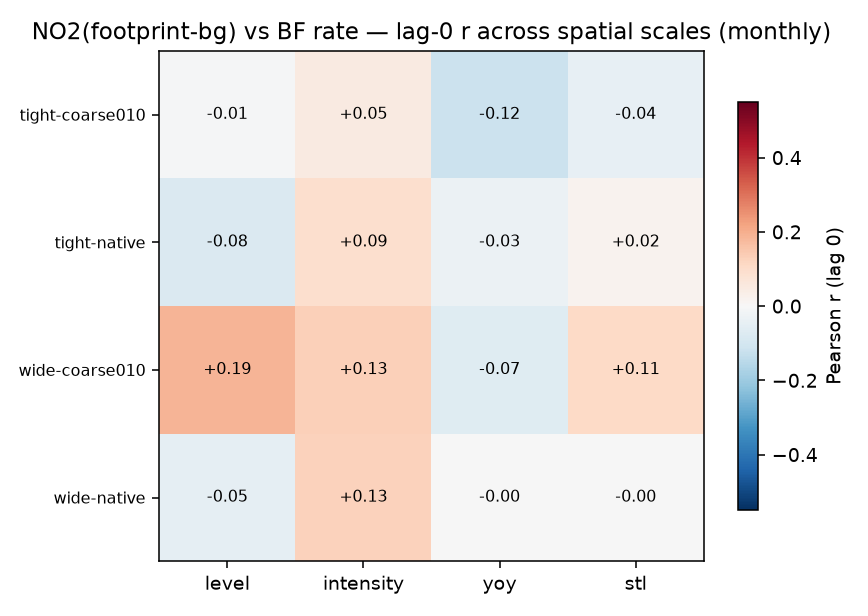
\includegraphics[width=0.74\linewidth]{fig1_scale_r_heatmap.png}
\caption{Lag-0 Pearson $r$ between the meteo-normalised footprint$-$background \ce{NO_2} and the
BF operating rate across the four resolvable scales (rows) and four deseason variants (columns).
All $|r|<0.2$; the sign of the \textsf{level} relationship even flips between \textsf{wide-native}
($-0.05$) and \textsf{wide-coarse010} ($+0.19$).}
\label{fig:heatmap}
\end{figure}

\subsection{Serial dependence inflates the naive test}
Figure~\ref{fig:shrinkage} plots the autocorrelation-robust block-permutation $p$ against the
naive i.i.d.\ $p$ for every cell. Points sit on or above the diagonal: the honest $p$ is never
smaller than the naive one. The effective sample size (Table~\ref{tab:grid}) shrinks the nominal
$n=90$ to $n_{\text{eff}}\approx62$--$86$ --- a $5$--$31\%$ loss of independent information ---
and the \textsf{yoy} variant, which differences the series, loses the most. In this dataset the
naive test happens to agree (nothing is significant either way), but the gap is the general
warning: a single fixed-scale Pearson $p$ near $0.05$ on these series would be a false positive.

\begin{figure}[t]
\centering
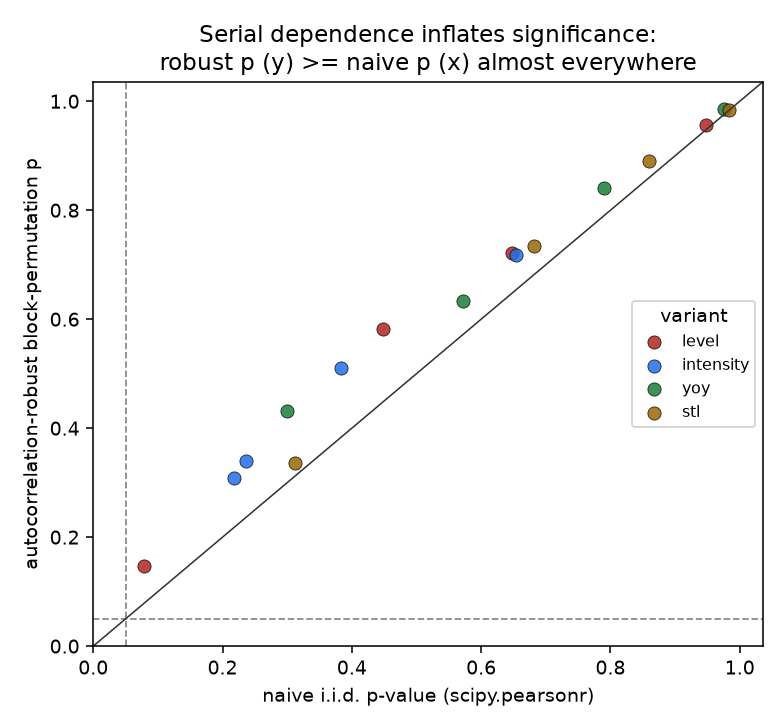
\includegraphics[width=0.52\linewidth]{fig2_neff_shrinkage.png}
\caption{Autocorrelation-robust $p$ (block permutation) vs the naive i.i.d.\ $p$
(\texttt{scipy.pearsonr}) for all $16$ cells. Every point lies on or above the $45^{\circ}$ line:
serial dependence can only \emph{inflate} significance, never deflate it. Dashed lines mark
$p=0.05$.}
\label{fig:shrinkage}
\end{figure}

\subsection{The levels coupling is weak and sign-unstable}
Figure~\ref{fig:forest} is a forest plot of the bootstrap CIs for the \textsf{level} variant
across scales. Every interval crosses zero, and the point estimates change sign with scale
($-0.05,+0.19,-0.08,-0.01$). The negative ``decoupling'' levels relationship that read
$\sim-0.35$ on the partial cube is, on the complete cube, a near-zero estimate whose sign is not
even stable to the AOI buffer or the grid factor. Figure~\ref{fig:decoupling} shows why directly:
the BF rate climbs steadily while the meteo-normalised cluster \ce{NO_2} hovers around zero with
no matching trend --- visual decoupling, \rval{-0.05}, $n=90$.

\begin{figure}[t]
\centering
\begin{subfigure}[t]{0.49\linewidth}
\centering
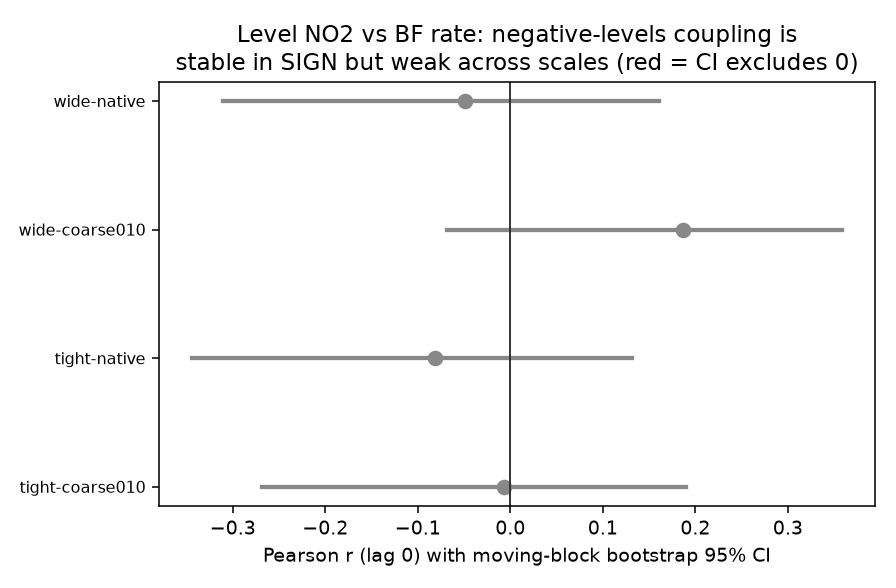
\includegraphics[width=\linewidth]{fig3_level_forest.png}
\caption{Bootstrap 95\% CI of $r$ (\textsf{level}) across scales; all cross zero.}
\label{fig:forest}
\end{subfigure}\hfill
\begin{subfigure}[t]{0.49\linewidth}
\centering
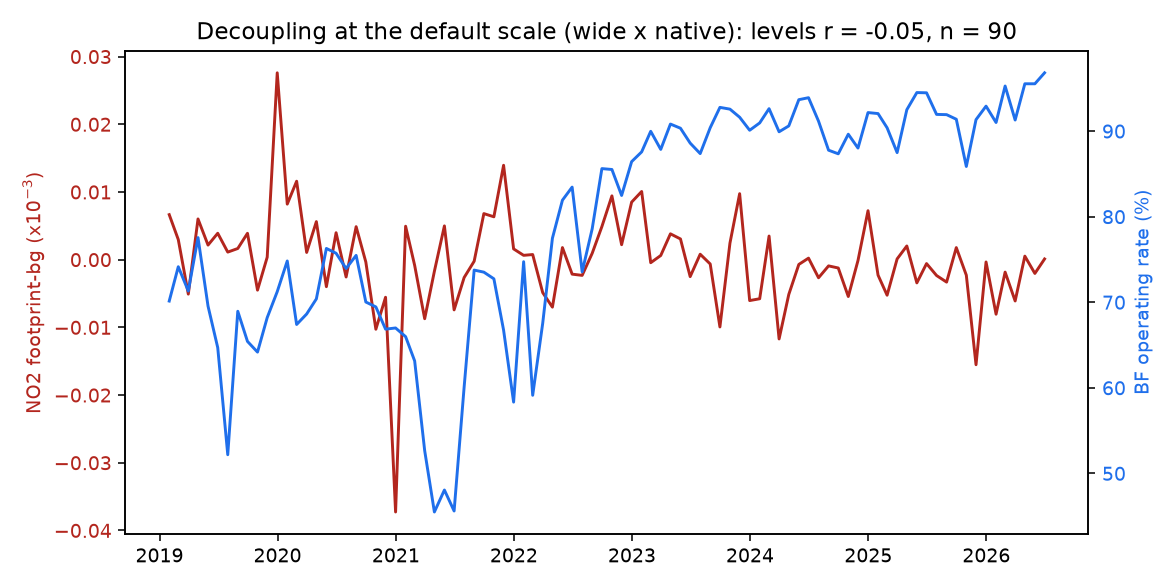
\includegraphics[width=\linewidth]{fig4_decoupling.png}
\caption{Default scale: BF rate (blue) trends up; \ce{NO_2} (red) is flat.}
\label{fig:decoupling}
\end{subfigure}
\caption{The levels relationship at and across the default scale. Left: the moving-block
bootstrap CI of the lag-0 $r$ for the \textsf{level} variant at every resolvable scale ---
each interval includes zero, and the central estimate changes sign. Right: the monthly time
series at the default (\textsf{wide}\,$\times$\,\textsf{native}) scale.}
\label{fig:levels}
\end{figure}

\subsection{Regime dependence, not a stable signal}
The only place the coupling is ever strong is \emph{locally in time}. Figure~\ref{fig:rolling}
shows the $18$-month rolling correlation of the \textsf{level} and \textsf{intensity} variants
against the BF rate at the default scale: it wanders between strongly positive and strongly
negative without settling. A rolling window will always surface a transiently high $|r|$ in a pair
of autocorrelated series; that is a property of the estimator, not evidence of a usable signal,
and it is precisely why the full-window, scale-swept, FDR-corrected test in
Table~\ref{tab:grid} is the appropriate arbiter.

\begin{figure}[t]
\centering
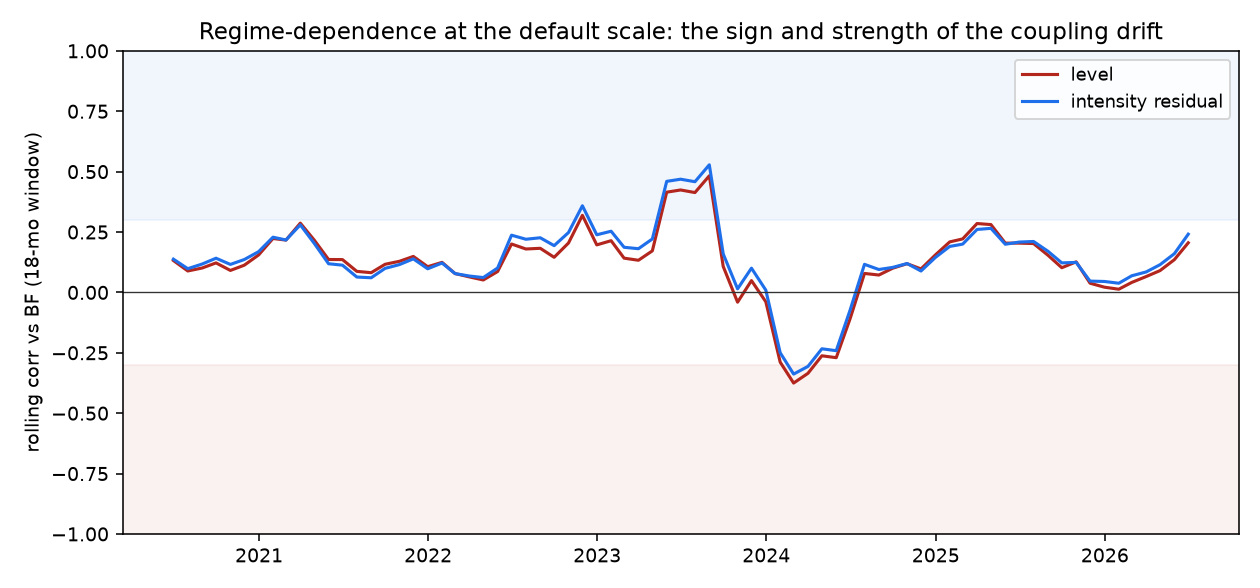
\includegraphics[width=0.82\linewidth]{fig5_rolling_regime.png}
\caption{18-month rolling correlation vs the BF rate at the default scale for the \textsf{level}
(red) and \textsf{intensity}-residual (blue) variants. The sign and strength drift across regimes;
no stable coupling emerges. Shaded bands mark $|r|\ge0.3$.}
\label{fig:rolling}
\end{figure}

\subsection{The coarsest grid cannot resolve a source contrast}
At $\sim$\SI{0.25}{\degree} ($\sim$\SI{25}{km} cells) the footprint/background geometry collapses:
within the clipped AOI the background ring (inner $\sim$\SI{71}{km}, outer $\sim$\SI{106}{km} once
floored to the coarse cell size) contains no cells, for both the wide and the tight extent
(\texttt{GeometryError}, ERR-003). This is itself the \citet{parubets_naito_2025} warning in its
strongest form: at a coarse enough resolution the cluster and its background are no longer
separable objects, so the source-isolation signal is undefined, not merely weak. The two
\textsf{coarse025} scales are therefore reported as \emph{not resolvable} rather than forced, and
the grid in Table~\ref{tab:grid} comprises the four scales that admit a valid contrast.

\section{Discussion}
\label{sec:discussion}

\paragraph{The null is robust to both suspicions.} Neither a tighter AOI (less BTH background
dilution) nor a coarser grid (more spatial aggregation) rescues the coupling, and the
autocorrelation-aware test --- which can only \emph{reduce} significance --- does not promote any
cell. The weak/null \ce{NO_2}$\leftrightarrow$BF relationship is not a fixed-scale artefact and not
an i.i.d.-inflation artefact. The earlier $-0.35$ ``decoupling'' was a feature of the partial cube;
the complete 389-week series collapses it to $-0.05$, consistent with the documented full-series
arbiter (weekly $0.07$, monthly $0.13$).

\paragraph{Why a level estimator is capped here.} Steel is only $\sim$30--43\% of the Tangshan
\ce{NO_2} column \citep{scirep_2024}; traffic, power and residential sources fill the rest, and the
ultra-low-emission retrofit programme drives a secular intensity decline that decouples emissions
from output \citep{li_2024_nox_trends}. With steel a minority, season-dependent share of a noisy
column \citep{montgomery_holloway_2018}, a level-correlation estimator faces a signal-to-noise
ceiling that more spatial slicing of a single daily overpass cannot lift. This is the same ceiling
NOX-006 hit from the temporal side: TROPOMI's lone $\sim$13:30 sample cannot separate baseload steel
from the cyclical traffic that would otherwise be removed by a day-of-week term.

\paragraph{Methodological takeaway.} The experiment also demonstrates a discipline worth keeping:
sweeping scale \emph{and} lag multiplies the number of tests, and any single ``significant'' cell
must be read against that multiplicity. The combination of a moving-block bootstrap, a
block-permutation null, and a Benjamini--Hochberg correction \citep{morris_zhang_2019} converts a
tempting collection of $|r|\!\sim\!0.3$ peak-lag values into the honest conclusion they deserve.

\paragraph{What could still move the needle.} Two levers remain, both outside this paper's
aggregation-only scope. (i) A \emph{diurnal} sensor: GEMS, the geostationary spectrometer over East
Asia, samples $\sim$8 times per day and could resolve the weekday cycle that separates flat steel
baseload from cyclical traffic, lifting steel's \emph{variance} share above the mean-share ceiling
\citep{park_2025_gems_gan}. (ii) \emph{Flux-divergence} point-source attribution
\citep{beirle_2021,beirle_2023}, which isolates the local source term from the regional background
physically rather than statistically --- known to be hard in high-background, complex-wind
industrial NE China, which is exactly why it is sequenced after a relative-index null is
established. NOX-008's robust null is the go-signal that a relative-index, single-overpass approach
has been exhausted at this cluster.

\section{Conclusion}
\label{sec:conclusion}
On the complete TROPOMI cube, the Tangshan steel-activity \ce{NO_2} signal shows no robust
correlation with the blast-furnace operating rate at \emph{any} reasonable spatial scale, under an
autocorrelation-aware, multiple-testing-corrected test: $0/16$ cells significant, sign-unstable in
levels, and undefined at the coarsest grid. The result is not a failure of the pipeline but a
sharpened, defensible boundary on what a single-overpass relative-index method can deliver for one
industrial cluster --- and a clean motivation for the diurnal-sensor and flux-divergence phases that
follow.

\paragraph{Reproducibility.} All figures and Table~\ref{tab:grid} are produced by
\texttt{analysis/nox008\_spatial\_scale.py} (seed $20260614$, $5000$ bootstrap/permutation draws),
reading \texttt{data/derived/no2/no2\_cube\_w.nc} (gitignored) and
\texttt{data/derived/benchmark\_tangshan\_bf\_operating\_rate.parquet}. Outputs:
\texttt{docs/figures/nox008/}. \ce{NO_2}-derived artefacts are gitignored; the stats table and
figures are committable.

\begin{thebibliography}{99}
\setlength{\itemsep}{0.15em}

\bibitem[Beirle et al.(2021)]{beirle_2021}
S.~Beirle et al.
\newblock Catalog of \ce{NO_x} emissions from point sources as derived from the divergence of the
\ce{NO_2} flux for TROPOMI.
\newblock \emph{Earth Syst. Sci. Data}, 13:2995--3015, 2021.

\bibitem[Beirle et al.(2023)]{beirle_2023}
S.~Beirle et al.
\newblock Improved catalog of \ce{NO_x} point source emissions (version 2).
\newblock \emph{Earth Syst. Sci. Data}, 15:3051--3073, 2023.

\bibitem[C3S CDS(2026)]{cds_era5}
Copernicus Climate Change Service (C3S), Climate Data Store.
\newblock ERA5 hourly data on single levels (\texttt{reanalysis-era5-single-levels}), 2026.
\newblock CDS API, accessed 2026-06-13.

\bibitem[CREA(2026)]{crea_steel_benchmark}
Centre for Research on Energy and Clean Air.
\newblock China steel-sector operating-rate series (incl.\ Tangshan blast-furnace operating rate),
2026. Public CSV export; accessed 2026-06-13.

\bibitem[Donaldson and Storeygard(2016)]{donaldson_storeygard_2016}
D.~Donaldson and A.~Storeygard.
\newblock The view from above: applications of satellite data in economics.
\newblock \emph{J. Econ. Perspect.}, 30(4):171--198, 2016.

\bibitem[Ezran et al.(2023)]{ezran_2023}
I.~A.~S. Ezran, S.~D. Morris, M.~G. Rama, and D.~Riera-Crichton.
\newblock Measuring global economic activity using air pollution.
\newblock World Bank Policy Research Working Paper 10445, 2023.

\bibitem[Hersbach et al.(2020)]{hersbach_2020_era5}
H.~Hersbach et al.
\newblock The ERA5 global reanalysis.
\newblock \emph{Q. J. R. Meteorol. Soc.}, 146(730):1999--2049, 2020.

\bibitem[Kim et al.(2023)]{kim_2023}
J.~Kim et al.
\newblock A systematic approach to identify shipping emissions using spatio-temporally resolved
TROPOMI data.
\newblock \emph{Remote Sens.}, 15(13):3453, 2023.

\bibitem[Li and Zheng(2023)]{li_zheng_2023}
H.~Li and B.~Zheng.
\newblock TROPOMI \ce{NO_2} shows a fast recovery of China's economy in the first quarter of 2023.
\newblock \emph{Environ. Sci. Technol. Lett.}, 10(8):635--641, 2023.

\bibitem[Li et al.(2024)]{li_2024_nox_trends}
H.~Li et al.
\newblock Trends and drivers of anthropogenic \ce{NO_x} emissions in China since 2020.
\newblock \emph{Environ. Sci. Ecotechnol.}, 21:100425, 2024.

\bibitem[Mao et al.(2025)]{mao_2025_ukraine}
Y.~Mao et al.
\newblock Inversion-based assessment of anthropogenic \ce{NO_x} emission changes in Ukraine during
the 2022--2023 war using TROPOMI.
\newblock \emph{Atmos. Chem. Phys.}, 25:14187--14204, 2025.

\bibitem[Montgomery and Holloway(2018)]{montgomery_holloway_2018}
A.~Montgomery and T.~Holloway.
\newblock Assessing the relationship between satellite-derived \ce{NO_2} and economic growth over
the 100 most populous global cities.
\newblock \emph{J. Appl. Remote Sens.}, 12(4):042607, 2018.

\bibitem[Morris and Zhang(2019)]{morris_zhang_2019}
S.~D. Morris and J.~Zhang.
\newblock Validating China's output data using satellite observations.
\newblock \emph{Macroecon. Dyn.}, 23(8):3327--3354, 2019.

\bibitem[Park et al.(2025)]{park_2025_gems_gan}
J.-E. Park, Y.-J. Choi, G.~Kim, and S.~Hong.
\newblock Real-time nowcasting of \ce{NO_2} products from GEMS using a conditional GAN.
\newblock \emph{Atmos. Pollut. Res.}, 16(10):102631, 2025.

\bibitem[Parubets and Naito(2025)]{parubets_naito_2025}
S.~Parubets and H.~Naito.
\newblock Predicting economic activity using atmospheric \ce{NO_2} satellite data: evidence from
local economic indicators in Japan.
\newblock \emph{PLOS ONE}, 20(12):e0337901, 2025.

\bibitem[Sci. Rep.(2024)]{scirep_2024}
Analysis of the synergistic benefits of typical technologies for pollution and carbon reduction in
the iron and steel industry in the Beijing--Tianjin--Hebei region.
\newblock \emph{Sci. Rep.}, 14, 2024. doi:10.1038/s41598-024-63338-8.

\end{thebibliography}

\end{document}
